\documentclass[11pt, english]{article}
\usepackage{graphicx}
\usepackage[colorlinks=true, linkcolor=blue]{hyperref}
\usepackage[english]{babel}
\selectlanguage{english}
\usepackage[utf8]{inputenc}
\usepackage[svgnames]{xcolor}
\usepackage{afterpage}
\pagestyle{plain}
\usepackage{here}
\usepackage{color}
\usepackage{ragged2e}
\usepackage{booktabs}
\usepackage{verbatim}

\begin{document}
\begin{center}
\vspace*{-1in}
\begin{figure}[htb]
\begin{center}

\includegraphics[width=8cm]{logo.png}
\end{center}
\end{figure}
\begin{large}
\sc{Department of Data Science}\\
\end{large}
\vspace*{0.2in}
\begin{Huge}
\sc{The Effectiveness of Stay Home Orders to Reduce COVID-19 Prevalence}\\
\end{Huge}
\vspace*{0.3in}
\begin{Large}
Anthony Song\\
Michael Egle\\
John Chandara\\
Jaydon Cobb\\
\end{Large}
\vspace*{0.3in}
\today\\
\end{center}
\newpage
\begin{center}
\begin{large}
\section*{Abstract}
The purpose of this investigation is to provide insight into how the citizens of the United States and the world responded to social distancing regulations, and effective how these rules have been. We also contrast the United States’ situation with other countries and elucidate trends that are produced by countries successfully suppressing the spread and deadliness of COVID-19. Using the mobility data provided by Apple and various global immunology statistics we were able to develop answers for the questions above.
\end{large}
\end{center}
\newpage
\section{Background}
Coronavirus disease 2019 (COVID-19) is an infectious disease caused by severe acute respiratory syndrome coronavirus 2 (SARS-CoV-2). Common symptoms include fever, cough, fatigue, shortness of breath and loss of smell. The disease was first identified in December 2019 in Wuhan, the capital of China's Hubei province, and has since spread globally, resulting in the ongoing 2019–20 coronavirus pandemic. The first case reported outside of China occurred in Thailand on January 13th, 2020, which spread from a woman traveling from the epicenter. As of April 29th, 2020, more than 3.17 million cases have been reported across 185 countries and territories, resulting in more than $224,000$ deaths. In mid-March of 2020, the COVID-19 disease began to spread like wildfire throughout the United States. As for the federal response to this outbreak, the cabinet of the president delegated all response and protection duties to the states’ governors. 
\subsection{Obtaining Our Data}
We obtained our data from three primary sources, The Apple Mobility Dataset\cite{apple}, New York Times COVID-19 Dataset\cite{NYT}, and the Worldometer Dataset\cite{worldometer}. The steps below highlight how we obtained and cleaned each dataset. 

\newpage
\subsection{Apple Mobility Data}
\begin{enumerate}
    \item Obtain the dataset.
    \item Pivot dataset to increase rows by creating a column containing the dates. 
    \item Change the date to year-month-date format using lubridate.
\end{enumerate}{}
\subsection{New York Times COVID-19 Dataset}
\begin{enumerate}
    \item Read in the data directly from the GitHub URL.
    \item Use the lubridate package to change the date column to type Date from character.
    \item Break the data into four subdivisions for the four cities of interest. The names of these four new data frames are \texttt{nyc}, \texttt{mia}, \texttt{chi}, and \texttt{sf}.
\end{enumerate}{}
\subsection{Worldometer Dataset}
\begin{enumerate}
    \item Obtain the dataset.
    \item The data is composed of death per million people Worldometer data for various countries on April 24th, 2020. Values were chosen after a preliminary comparison using Microsoft Excel. 
    \item Rate of decrease in mobility column data was calculated using a \texttt{stat\_smooth()} regression line. The rate calculated from the local max to the local minimum. 
    \item Apply first row as column names, then convert characters to numeric values. 
Take absolute values for plotting purposes.

\end{enumerate}{}\newpage
\section{Our Exploration}
\subsection{Hypothesis}
We wanted to look at the effects of staying inside on the spread of the virus and as a result, the deaths caused by the virus. In theory, if people stay home more, there will be fewer interactions and less chances to spread the virus. Our group made the decision to use deaths as our statistic to show the spread of the virus rather than cases. We did this for a variety of reasons. First, this virus is much worse than a common flu and businesses would not be shutting down entirely if not for the tens of thousands of deaths across the country. Second, some regions are testing their citizens much more regularly than others. Third, it’s not uncommon for people to have the virus and never show symptoms at all. We attempted to simultaneously visualize the change in mobility in our data along with the number of new deaths reported each day.
\begin{figure}[h!]
  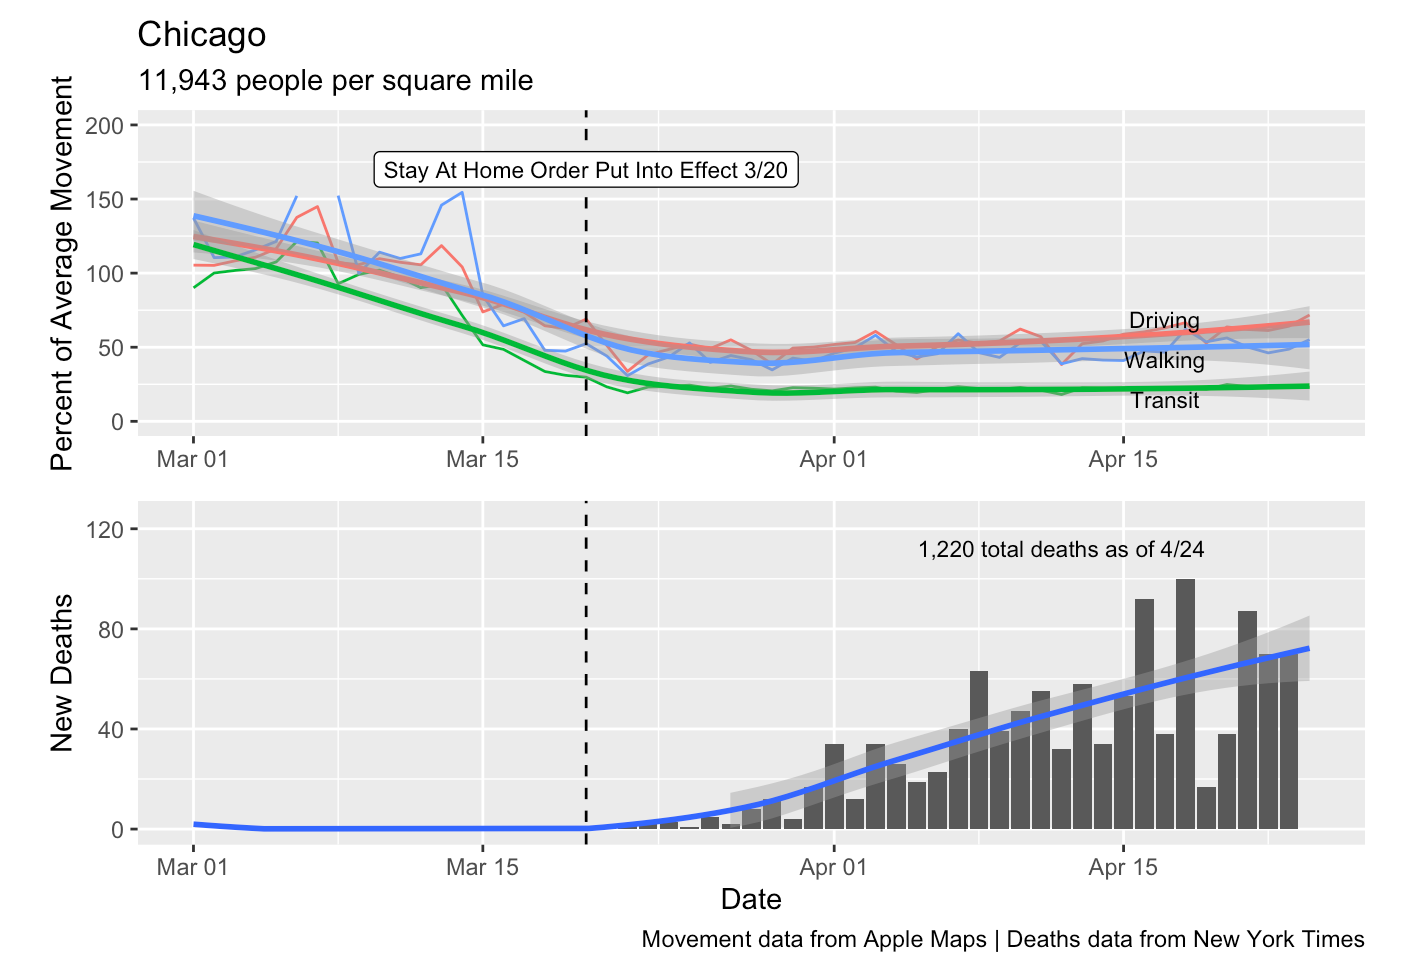
\includegraphics[width=\linewidth]{image6.png}
  \caption{Change in mobility plotted with number of daily new deaths for Chicago, IL}
  \label{fig:chicago}
\end{figure}
\subsection{Case Study of Chicago, IL}
As an example, Chicago’s data is shown above in \textit{Figure 1}. The y-axis on the top half is the percentage of movement compared to an average day in the given region. As shown, there was a significant decrease in movement even before the stay at home order was officially put in place. However the numbers have slowly crept back towards the average, which may help to explain why the curve in Chicago still has not flattened.
\newpage
\subsection{Case Study of Other Regions}

\begin{figure}[h!]
  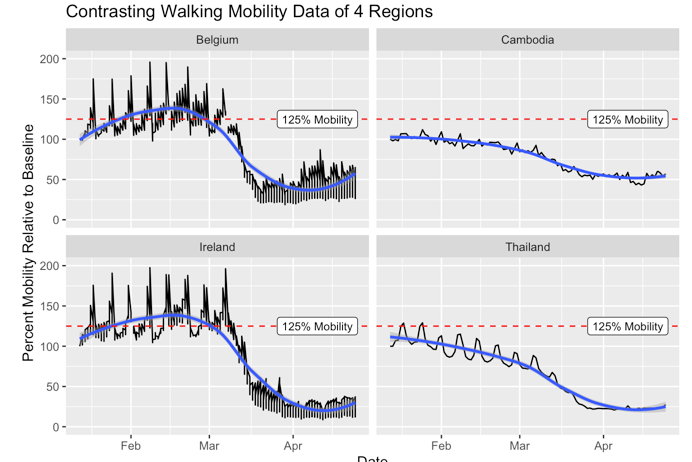
\includegraphics[width=\linewidth]{image1.png}
  \caption{Comparison of mobility data for low death rate and high death rate regions}
  \label{fig:mobility}
\end{figure}

After looking at the US analysis, We wanted to further explore the mobility data and look for trends amongst other countries and regions. Similar to the first analysis, we started exploring the death data in order to reduce confounding variables, like individuals that were hypochondriacs (people that misdiagnose minor symptoms), that might be associated with the reported number of COVID-19 cases. After viewing many countries in the upper and lower median of the Worldometer data set for deaths per million people, we extracted five extreme values for low death rate (LDR) and high death rate (HDR) countries. Due to the mysterious nature of this virus, we thought it would be best to start looking for trends in the upper (Belgium/Ireland, \textit{Figure 2}) and lower (Cambodia/Thailand, \textit{Figure 2}) extremities, this would illuminate any potential correlations that may be unclear in countries with death rates around the median. We wanted to specifically target only the walking data, as this would provide a better representation of social interactions and potential interactions that occur within a six foot radius of another human. After plotting the relative walking mobility as a function of the date for each extracted country, we stumbled upon a trend that grouped the countries by their respective death rates as shown below.


Using \texttt{geom\_smooth} to statistically create a smooth trendline, we found that all of our LDR and HDR countries could be represented by either a shallow or steep sine curve for LDR and HDR respectively. We found the best distinguishing factor to quantify these inherently different functions would be to measure the decreasing rate of change found at the mid-February to April time frame. The rate of change was determined by the data points produced by the \texttt{geom\_smooth} regression line. We then measured the rate of change from the local maximum to the local minimum. We decided to look at the maximum and minimum of the regression line instead of the raw data because this would overlook any extreme values produced from highly mobile dates. Doing this for every extracted country, we obtained a data set that looked like \textit{Table 1}. (ddp)

\begin{table}[h!]
\centering
\begin{tabular}{p{0.18\textwidth}p{0.18\textwidth}p{0.18\textwidth}p{0.18\textwidth}} \\ \toprule
\textbf{Country} & \textbf{Deaths per Million} & \textbf{Change in Mobility} & \textbf{Below 125\%} \\ \midrule
Indonesia & 3 & -1.4512530 & 1\\
Cambodia & 0 &-0.7241492 & 1 \\
Korea & 5 & -1.5005610 & 1 \\
Taiwan & 0.3 & -0.5122063 & 1 \\
Thailand & 0.71 & -1.2754960 & 1 \\
Italy & 426 & -2.6000790 & 0 \\
United Kingdom & 299 & -2.1510730 & 0 \\
Spain & 490 & -3.5016930 & 0 \\
Belgium & 597 & -2.7629390 & 0 \\
Ireland & 215 & -2.6594180 & 0 \\\bottomrule
\end{tabular}
\caption{Data Set with the country, death rate, decreasing mobility rate and below $125\%$ mobility, which is referred to as dpp.}
\end{table}
\clearpage
\subsection{Statistical Implications}
\begin{figure}[h!]
  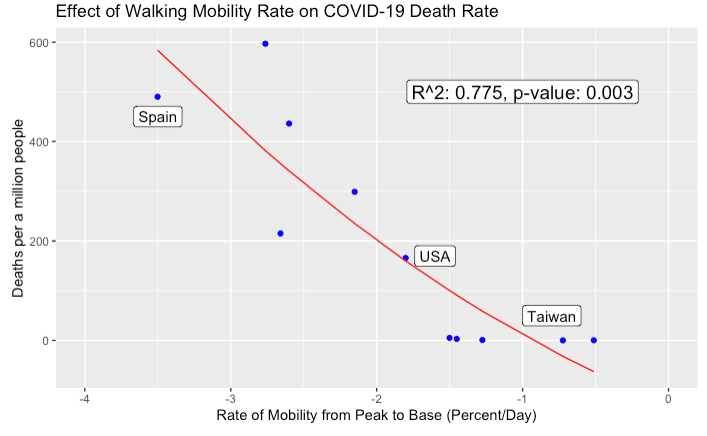
\includegraphics[width=\linewidth]{image4.png}
  \caption{Regression model of death million people as a function of decreasing mobility}
  \label{fig:regression}
\end{figure}

While exploring the rate of change we noticed another trend that was intrinsic to LDR and HDR countries, the frequency of mobility percentages above $125\%$. Intuitively, high frequency of dates with high mobility is bound to spread bacteria quickly,  but we did not continue this exploration because after preliminary tests, we found that these values did not show much promise in correlation. From \textit{Table 1}, we plotted the deaths per million as a function of decreasing rate in mobility for all countries. The graph seemed to show a polynomial trend and after some regression fitting using the \texttt{lm()} function, we were able to obtain a model, as shown in \textit{Figure 3}, with a coefficient of determination ($r^2$) of $0.775$ and p-value of $0.003$ . This showed a promising trend that would help us answer our questions.
\clearpage
\section{Data Wrangling and Visualization}
\textbf{Important Notes}
\begin{enumerate}
    \item Most data is prepared and plotted using dplyr pipeline ($\%>\%$).
    \item Annotations on visualizations are prepared using annotate() function.
\end{enumerate}

\subsection{Preparation}
\begin{enumerate}
    \item Change the dates to rows so we can plot the data efficiently.
    \item Change the date values to year/month/date to increase accessibility.
    \item Use the filter function to extract specific walking and country data, then bind the specific sets into a new data set. 
\end{enumerate}

\subsection{Data Visualization Preparation}
In order to show how the mobility data and new deaths per day data increased or decreased together over time, we put the plots on top of one another as seen above in \textit{Figure 1}. 

\begin{enumerate}
    \item Preparation of the top half of \textit{Figure 1}: The line plot represents the three types of mobility data that was provided by Apple: walking, driving, and transit. We separated these due to the fact that low levels of walking and transit use are more important than use of driving.
\begin{verbatim}
chi_travel_viz <- chi_travel %>% 
    ggplot(
        aes(
            x = date,
            y = percent_change,
            group = transportation_type,
            color = transportation_type
        )
    ) + 
    geom_line() +
    geom_smooth()
\end{verbatim}
\newpage
    \item Preparation of the bottom half of Figure 1: Histogram of each day’s newly reported deaths with a trend line to account for possible corrections in the data.
\begin{verbatim}
chi_deaths_viz <- chi %>% 
    ggplot(
        aes(
            x = date, 
            y = new_deaths
            )
        ) +
    geom_histogram(
        stat = "identity"
    ) + 
    geom_smooth()
\end{verbatim}

    \item Combination of plots: We utilized the ggpubr package for its \texttt{ggarrange} function, giving the user the ability to combine two plots on top of one another. In doing this, we now have a plot with corresponding x-axes for the top and bottom.
\begin{verbatim}
ggarrange(
    chi_travel_viz, 
    chi_deaths_viz, 
    nrow = 2
)
\end{verbatim}
\end{enumerate}
\newpage
\subsection{Data Visualization (Figure 2 \& 3)}
\begin{enumerate}
    \item Preparation of \textit{Figure 2}: Line graph of multiple countries mobility data with a regression line using facet\_wrap (\textit{figure 2})
\begin{verbatim}
qplot(date, percent_change, date = indo)
    + stat_smooth(aes(
        outfit = indo_tha<<-..y..
    ))
\end{verbatim}
    \item Rate of change graph and calculation for each country.
\begin{verbatim}
indo_tha <- data.frame(indo_tha)

fit_indo$day = seq.int(nrow(fit_indo))

vc_indo <- c(max(
        fit_indo$fit_indo),
        min(fit_indo$fit_indo)
    )
    
Max_min_indo <-
    fit_indo[fit_indo$fit_indo %in% vc_indo, ]
    
Rate_of_Change <- 
    (max_min_indo[2,1] - max_min_indo[1,1]) /
    (max_min_indo[2,2] - max_min_indo[1,2])
\end{verbatim}
\newpage
    \item Preparation of \textit{Figure 3}: Death rate of country as a function of mobility rate with a polynomial regression,  $r^2$ and p-value statistics.
\begin{verbatim}
regression = lm(
    dpp$’Deaths per a million people’ ~
    poly(
        dpp$’Rate of decrease in Mobility’,
        2,
        raw = TRUE
    ),
    data = dpp
)

pred_dpp <- data.frame(
    death = predict(regressor, dpp),
    rate = dpp$`Rate of decrease in Mobility`
)

summary(regression) # r^2 and p-value

ggplot(
    data = dpp,
    aes(
        y = `Death per a million people`,
        x = `Rate of decrease in Mobility`
    )) + 
    geom_line(
        color = `red`,
        data = pred_dpp, 
        aes(x = rate, y = death)
    )
\end{verbatim}
\end{enumerate}
\clearpage
\section{Discussion}
Using the Apple Mobility data, New York Times COVID-19 GitHub data, and Worldometer data we strove to answer four important questions: Have citizens obeyed social distancing regulations? Has it been effective? How are we (United States) handling this compared to other regions? What can we learn from regions that are successfully keeping COVID-19 prevalence low?
\subsection{Remarks on America's Response}
Starting off, we wanted to take a look into how the citizens of the United States are coping with the new regulations on social interaction. In the scope of this project, we answered this by looking at four large cities: New York City, Chicago, Miami and San Francisco. For these four cities, we can confirm that a vast majority of these citizens are obeying the government implemented social distancing regulations. This can be qualitatively and quantitatively observed by an intense decrease in walking, driving and transit mobility for the four cities. Furthermore, by incorporating the death toll, population density and the “Stay at Home Order” implementation date, we can draw conclusions on the regulation’s effectiveness. Based on these four cities, we can see that San Francisco had the most effective implementation of social distancing regulations. With the second highest population density, San Francisco, as of April 24th, 2020, kept their death toll to 22, which is extremely low compared to New York City (11,157 deaths) and Chicago (1,220 deaths). Outside of the mobility data, a factor that may explain San Francisco’s effective regulations is the well-timed implementation date. Compared to the other cities, San Francisco mandated their regulations at least 4 days before the other cities. This shines light on the effectiveness of early action in a global pandemic. 
\clearpage
\subsection{Remarks on Other Responses}
\begin{figure}[h!]
  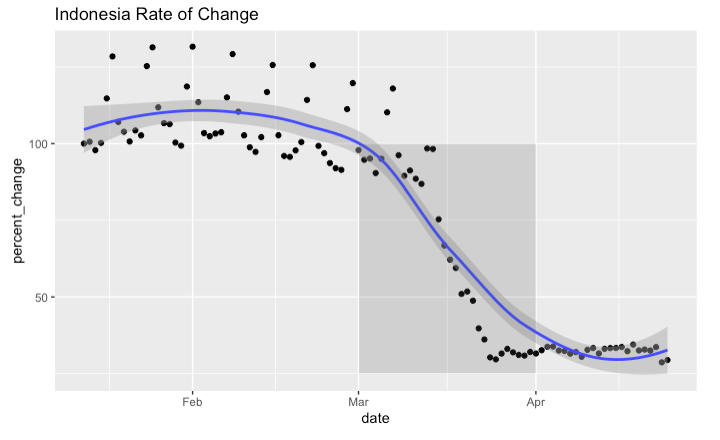
\includegraphics[width=\linewidth]{image3.png}
  \caption{Graph of Indonesia, regression line points were extracted for calculations of rate of change (ROC). The shaded region represents the region in which ROC was extracted.}
  \label{fig:regression}
\end{figure}
Broadening the scope of our regional analysis, we wanted to understand how the United States was battling this virus compared to the rest of the world. To answer this we looked at the relative death rate, percent mobility and decreasing rate of mobility. Qualitatively, we observed the trends of mobility spikes that occurred from mid-February to early-March. These spikes reached values greater than 150\% the baseline mobility and follow similar trends of HDR regions like Ireland and Belgium shown in \textit{Figure 2}. Next we looked at the deaths per million people, which range from 0 to 597 (table1), the United States is in the middle at 166. Finally, we looked at the calculated decreasing mobility rate, which ranges from $-0.51$ to $-3.5$ (\textit{Table 1}) percent mobility per day, the United States is in the middle at -1.8. These values indicate that the United States is battling COVID-19 moderately, meaning our practices of containment could be improved. Digging deeper, we wanted to understand how we could quarantine more effectively, by learning from countries successfully battling the virus. We looked specifically at the five countries located in the bottom right corner of \textit{Figure 3}. These countries showed low death rate, mobility under $125\%$ of the baseline during mid-February to early-March and larger, and less-negative (shallow) rate of change. Our interpretation is that these countries were more inclined to react proactively at the beginning of this pandemic. These countries maintained their baseline mobility and slowly decreased it as the severity of the pandemic increased as seen by the mobility under $125\%$ and decreasing mobility rate respectively. Furthermore, this correlated to a low death rate and a statistically significant regression line ($\text{p-value} = 0.003$). Although we have shown this to be significant, it is important to understand this model may fail when generalized for all countries that lie between the extreme values. Fortunately, in our investigation, countries that took early action by implementing laws and reducing mobility early, analogous to San Francisco, were able to effectively contain this virus by consistently keeping their mobility, and potentially their social interactions, below their baseline values. 
\newpage
\section{Conclusion}

Amidst the chaos caused by an unexpected global pandemic, researchers in all fields have been collaborating to understand the physiological, sociological and economic pathology of this unknown virus. To join this mysterious expedition, we wanted to look into new datasets that might uncover valuable information. Using the Apple mobility, New York Times COVID-19 and Worldometer data, we were able to unveil potential trends on how citizens have obeyed social distancing regulations, the effectiveness of these regulations and what we can learn from countries successfully battling this virus. Looking into four densely populated cities in the United States we were able to uncover the effectiveness of early action as displayed by San Francisco, a city that had a relatively high population density and an extremely low death toll. San Francisco shows, compared to Chicago, Miami and New York City, that the early implementation of the “Stay at Home” order may have decreased the relative mobility of the city’s residents, in turn decreasing the spread of the disease and ultimately, lowering the death toll. Zooming out to a global level we found there was a correlation between periodic spikes of high mobility percentage, large decreasing rates in mobility around the time of panic (March-April) and deaths per million people (dpp) for various regions. Cities with high death rates (Belgium: $597$ dpp, Ireland: $215$ dpp), seemed to have frequent spikes of high mobility ($150-200\%$) at a crucial incubation period for the virus. These high moralities ultimately lead to more severe decreases in mobility when the virus starts to exponentially infect the residents. From these features and trends, we can conclude that countries and cities that followed social distancing regulations and to early action, benefited by maintaining a low death rate. In future studies, it may be important to study confounding variables, like culture, diet and immunity, that could possibly strengthen or weaken our claims. In the scope of our investigation, we believe that the mobility data has uncovered novel trends that help us understand the epidemiology of this mysterious Coronavirus. 
\newpage
\centering
\section*{Addendum}
This paper is dedicated to the hundreds of thousands of lives who have met an unfortunate demise to the horrible COVID-19 viral outbreak. May their souls rest in peace as we continue our efforts to fight this disease in an effort to save lives.
\newpage
\begin{thebibliography}{9}

\bibitem{apple} 
``COVID‑19 - Mobility Trends Reports.'' \textit{Apple}. 3 Jan. 2020,\\ www.apple.com/covid19/mobility.

\bibitem{andi} 
Burkert, Andi. ``Flattening the COVID-19 Curves.''\\\textit{Scientific American Blog Network}, Scientific American, 17 Mar. 2020,\\ blogs.scientificamerican.com/observations/flattening-the-covid-19-curves/.

\bibitem{NYT} 
The New York Times.\\``Coronavirus in the U.S.: Latest Map and Case Count.''\\
\textit{The New York Times}, The New York Times, 3 Mar. 2020,\\ https://github.com/nytimes/covid-19-data.

\bibitem{worldometer}
“Coronavirus Cases:” \textit{Worldometer}, www.worldometers.info/coronavirus/.

\end{thebibliography}
\end{document}